\section[Time Series]{时间序列预测}\label{sec:3}

\subsection[Modle]{时间序列模型}\label{subsec:3-1}

\begin{frame}
\ff{
	将所有采样段得到的$S_x$的分布的参数的第一个分量$\hat{\mu}_t( = X_t)$放在一起(其余分量同理),可以看作是一组取之于时间$t$的时间序列$\{X_1, X_2, \dots, X_T\}$的一个样本。而该时间序列可以看作如下数学模型\footcite{de1992some}:
\begin{equation}\label{TimeseriesModle}
	X_t = h(X_{t-1}, X_{t-2}, \dots, X_{t-p}, \epsilon_{t-1}, \epsilon_{t-2}, \dots, \epsilon_{t-q}) + \epsilon_{t}
\end{equation}
的一个抽样。其中$\{\epsilon_{t}\}$是一组独立同分布、有着共同均值$\mu$和共同方差$\sigma$的白噪声,一般而言,将样本数据中心化以后可以认为白噪声的均值$\mu = 0$。

\alert{目标:}根据$\{X_1, X_2, \dots, X_T\}$得到上式中$p$、$q$的估计,$h$的表达式的估计,和白噪声方差$\sigma$的估计。
}	
\end{frame}

\begin{frame}{ARIMA模型}
\ff{
	根据\cite{zhang2003time}的文献,我们可以分别用不同的模型来近似$h$的线性部分和非线性部分。$h$线性部分可以用ARIMA模型\footcite{box1994time}来近似:
	
	\begin{equation}\label{equ:ARIMA}
	LX_t + \sum_{i=1}^{p}\Phi_iX_{t-i} = \mu + \epsilon_t + \sum_{j=1}^{q}\theta_j\epsilon_{t-j}
	\end{equation}
	
	该模型的训练分为如下几个部分:
	\begin{enumerate}
	\item 数据平稳化:通常我们根据自相关系数趋于零的速度来判断数据的平稳性,如果数据是非平稳的,则通过差分将数据平稳化(一般差分的次数不超过两次)。
	\item 模型选择:根据\cite{box1994time},数据的自相关系数和偏自相关系数可以用于模型中参数$p$和$q$的选择。
	\item 参数拟合:选择了特定$p$和$q$以后,对$\Phi_i$、$\theta_j$、$\mu$的选择相当于利用非线性优化方法最小化预测值与真实值的误差
	\item 模型评估:我们可以事先留出部分数据作为验证集,利用白噪声检验,判断模型在验证集上的预测值与真实值之间的差是否是独立同分布的正态分布。如果没通过就返回第二步重新选取$p$和$q$,然后进行步骤三四。
\end{enumerate}
	
	如果数据具有周期性也可以添加上周期项使用季节性ARIMA模型。
}
\end{frame}

\begin{frame}{神经网络模型}
\ff{
	\cite{zhang2003time}提到利用人工神经网络ANN模型(公式(\ref{equ:ANN}))来近似非线性部分效果会很好。
	\begin{equation}\label{equ:ANN}
		y_t = \alpha_0 + \sum_{j = 1}^{q}\alpha_jg(\beta_{0j} + \sum_{i = 1}^{p}\beta_{ij}y_{t-i}) + \epsilon_t
	\end{equation}
	其中函数$g(x)$被称作激活函数,通常被取做logistic函数(公式(\ref{equ:logistic})),当然双曲正切函数$g(x) = a\tanh(bx)$或其他可行的函数也可以替代。
	\begin{equation}\label{equ:logistic}
		g(x) = \frac{1}{1 + \exp(-x)}
	\end{equation}
	
	真实值与ARMIA模型的预测值之间的误差可以作为神经网络模型的训练数据,模型的具体的训练步骤与ARIMA模型的第二到第四步类似,只不过第三步中对于表达式系数的预测一般可以用误差逆传播法、遗传算法\cite{montana1989training}......
}
\end{frame}

\begin{frame}{模型训练}
\ff{
	实际应用中,对于ARIMA模型的训练利用的是Python的库\textit{pmdarima},它是专门用来求解拟合ARIMA模型以及SARIMA模型的库,利用函数\textit{auto\_arima}可以便利地求出在当$p$和$q$限制在一定范围内时最优的$p$和$q$的估计值以及ARIMA模型相应系数。对于ANN模型的构建则使用的是\textit{keras}库,它相当于是一个神经网络API,有着用户友好、模块化程度高、扩展性好等优点,可以以\textit{TensorFlow}作为后端运行,速度也较快。
}
\end{frame}

\subsection[Sample]{时间序列算例}
\begin{frame}{时间序列算例}
\ff{
	我们选取澳大利亚的月啤酒生产量作为时间序列样本,下图反映出该序列有很强的季节性,波动规律大约是以一年为周期,因此我们采用季节性ARIMA模型与ANN模型的混合模型来进行预测。
	\begin{figure}[!htbp]
		\centering
		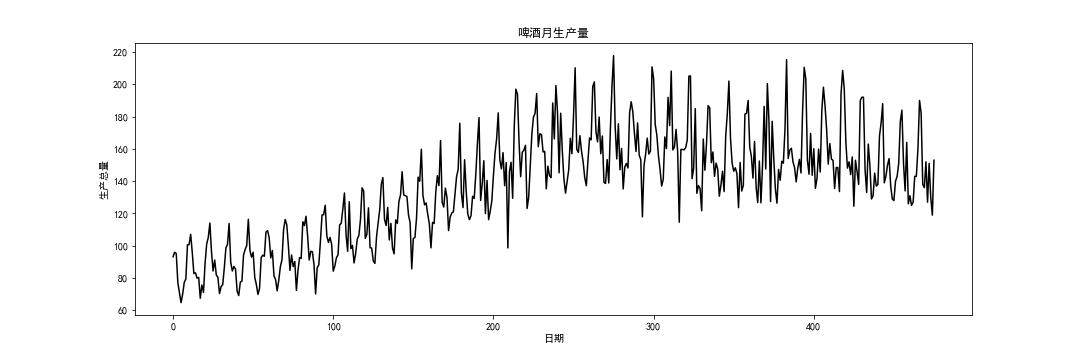
\includegraphics[width=5cm]{figure/monthly_beer_production}
		\caption{啤酒月生产量}
		\label{fig:monthly_beer_production}
	\end{figure}
	调用\textit{auto\_arima}函数,拟合得到最接近的模型为SARIMA$(3, 1, 3)\times(2, 0, 1, 12)$(即周期确实为$12$个月)。对于该种季节性数据,我们的混合的结果如下图\ref{fig:predictions3}。
	\begin{figure}[!htbp]
		\centering
		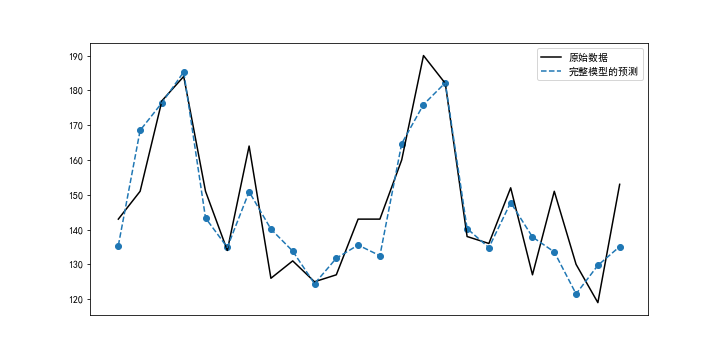
\includegraphics[width=5cm]{figure/predictions3}
		\caption{啤酒月生产量预测}
		\label{fig:predictions3}
	\end{figure}
	可以看到在验证集上我们的模型基本上很好拟合了实际数据。
}
\end{frame}
